%-----------------------------------LICENSE------------------------------------%
%   This file is part of Mathematics-and-Physics.                              %
%                                                                              %
%   Mathematics-and-Physics is free software: you can redistribute it and/or   %
%   modify it it under the terms of the GNU General Public License as          %
%   published by the Free Software Foundation, either version 3 of the         %
%   License, or (at your option) any later version.                            %
%                                                                              %
%   Mathematics-and-Physics is distributed in the hope that it will be useful, %
%   but WITHOUT ANY WARRANTY; without even the implied warranty of             %
%   MERCHANTABILITY or FITNESS FOR A PARTICULAR PURPOSE.  See the              %
%   GNU General Public License for more details.                               %
%                                                                              %
%   You should have received a copy of the GNU General Public License along    %
%   with Mathematics-and-Physics.  If not, see <https://www.gnu.org/licenses/>.%
%------------------------------------------------------------------------------%

%   Use the standalone class for displaying the tikz image on a small PDF.
\documentclass[crop, tikz]{standalone}

%   Import the tikz package to use for the drawing.
\usepackage{tikz}

%   Load the arrows.meta library.
\usetikzlibrary{arrows.meta}

%   Begin the document.
\begin{document}

    %   Draw the picture.
    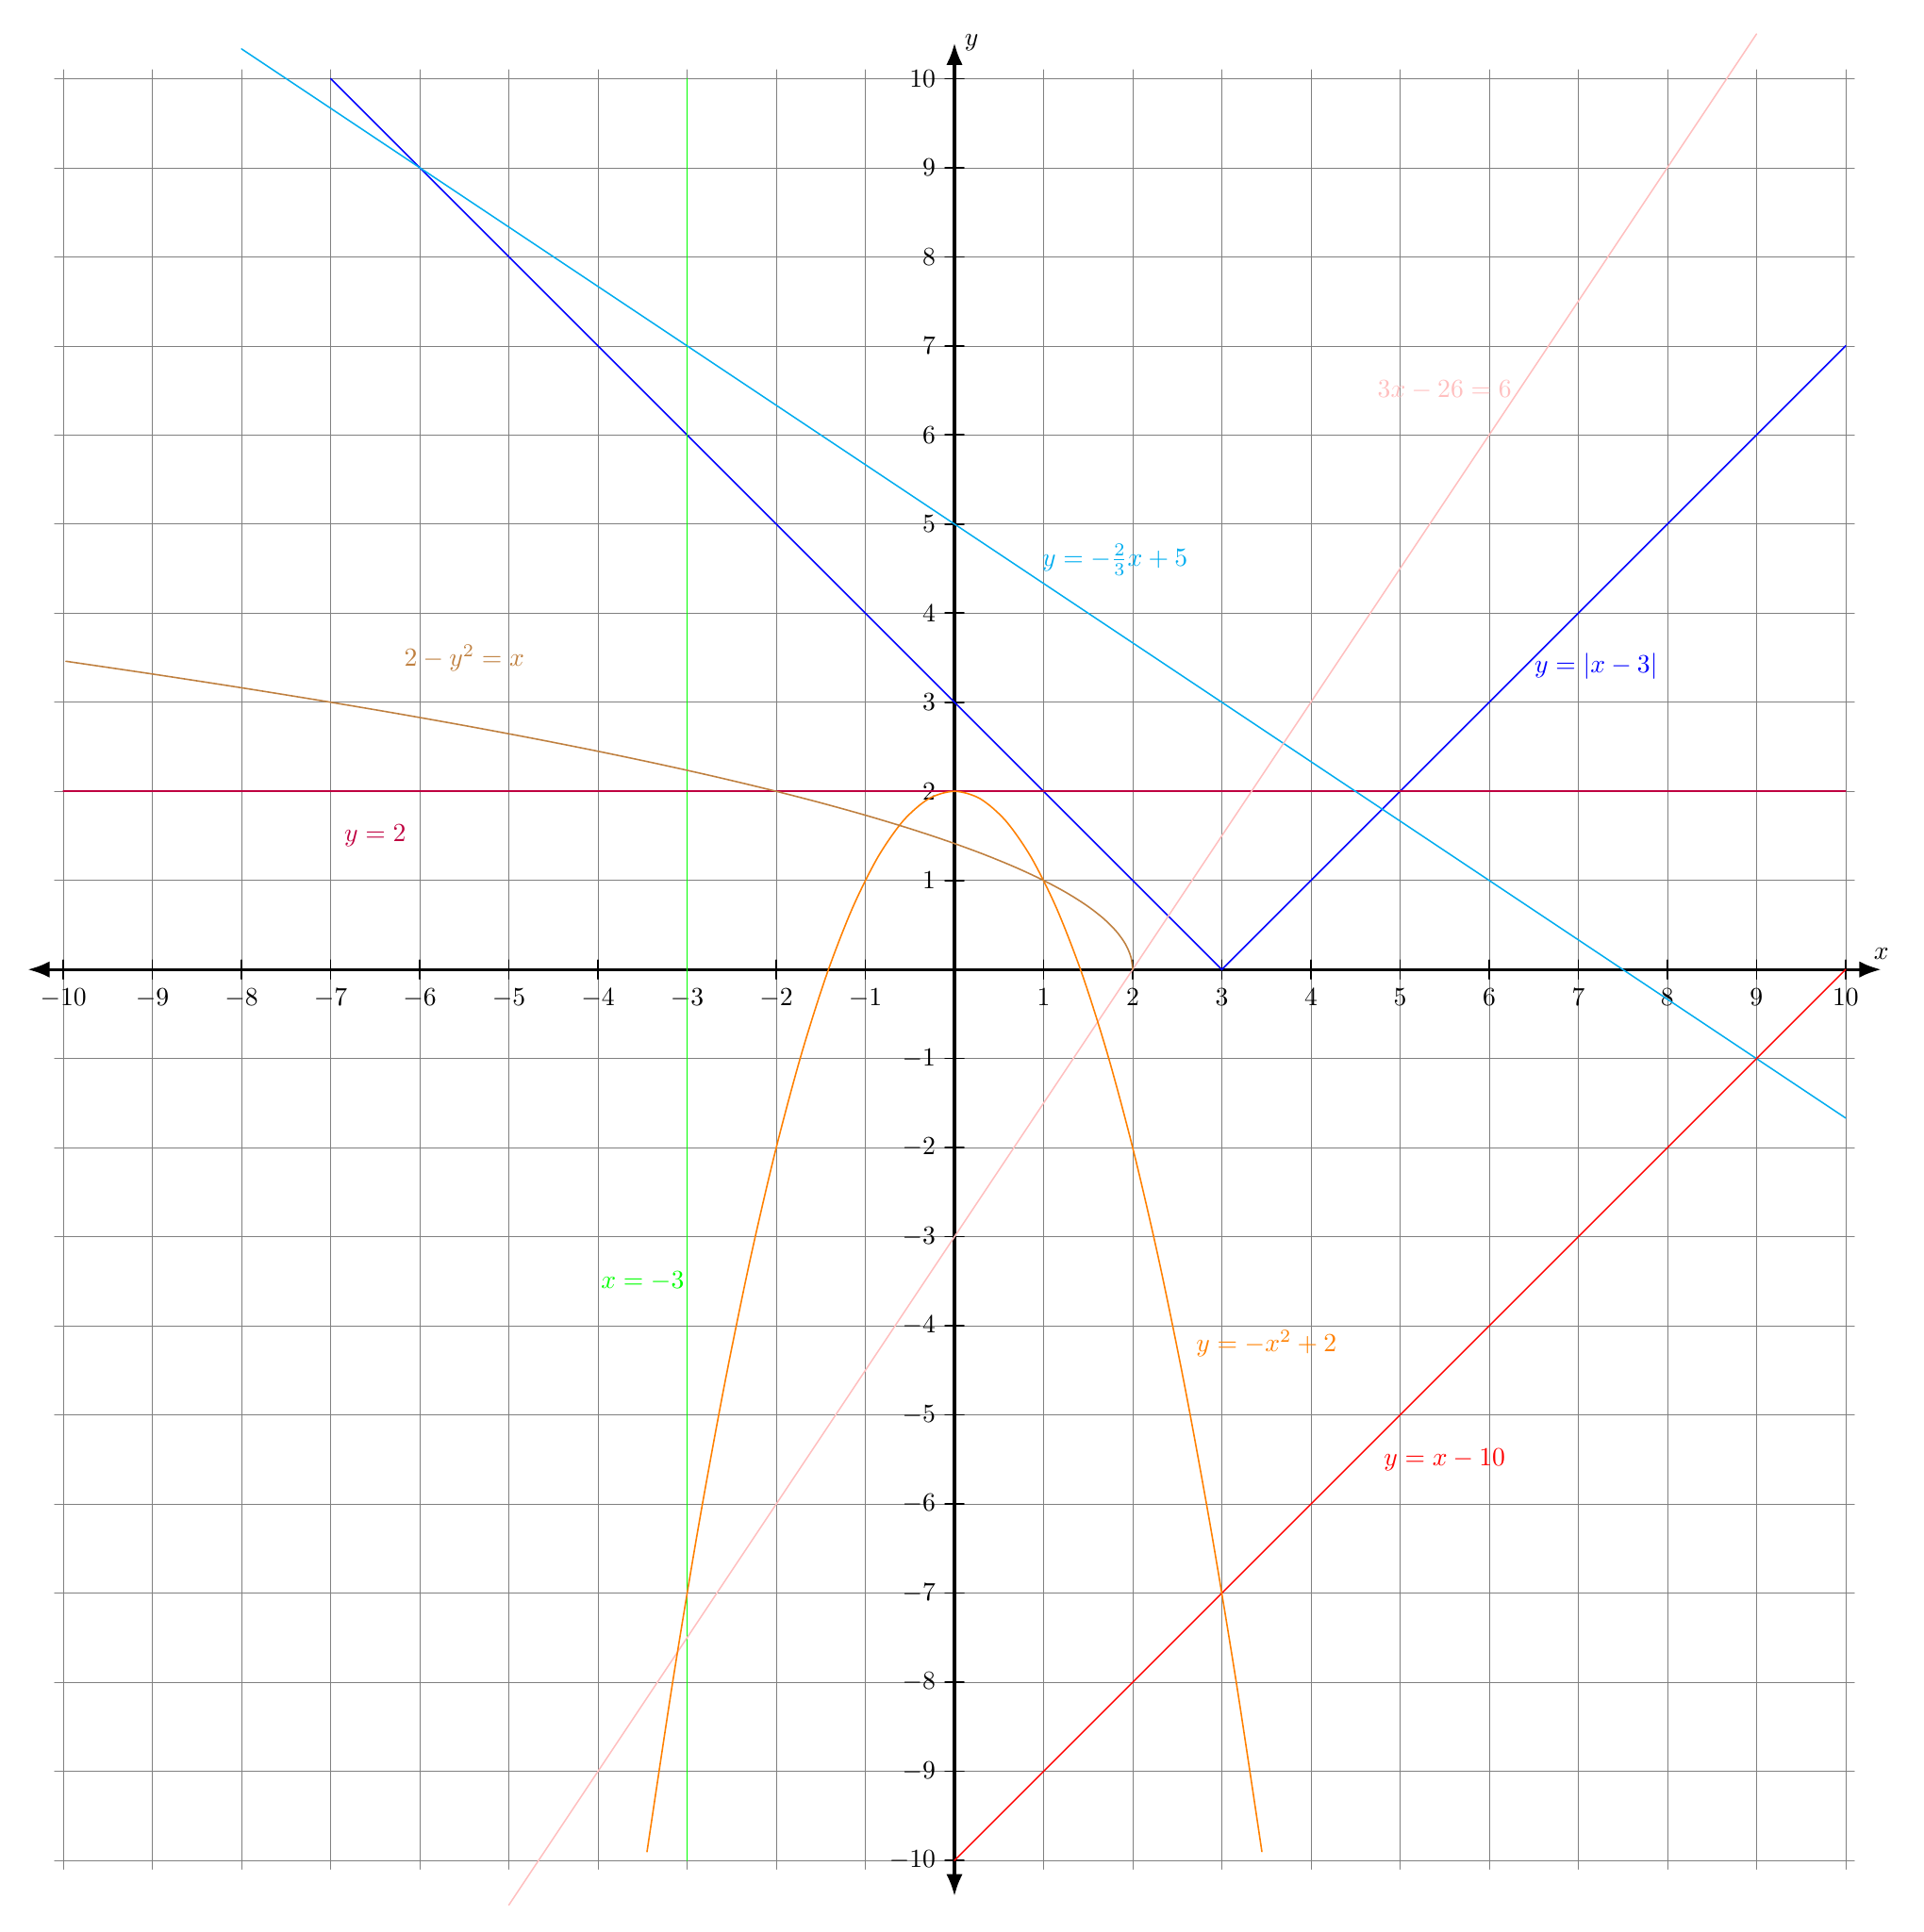
\begin{tikzpicture}[%
        >=Latex,
        line width=0.2mm,
        line cap=round,
        scale=1.2
    ]
        % Draw a grid.
        \draw[style=help lines] (-10.1, -10.1) grid (10.1, 10.1);

        % Axes.
        \begin{scope}[very thick]
            \draw[<->] (-10.4, 0.0) to (10.4, 0.0) node [above] {$x$};
            \draw[<->] (0.0, -10.4) to (0.0, 10.4) node [right] {$y$};
        \end{scope}

        % Axes labels.
        \foreach\n in {1, 2, ..., 10}{%
            \draw (\n, 3pt) to (\n, -3pt) node [below] {$\n$};
            \draw (-\n, 3pt) to (-\n, -3pt) node [below] {$-\n$};
            \draw (3pt, \n) to (-3pt, \n) node [left] {$\n$};
            \draw (3pt, -\n) to (-3pt, -\n) node [left] {$-\n$};
        }

        %   The absolute value function.
        \draw[draw=blue] (-7.0, 10.0) to (3.0, 0.0) to (10.0, 7.0);

        %   Straight lines.
        \draw[draw=green] (-3.0, -10.0) to (-3.0, 10.0);
        \draw[draw=purple] (-10.0, 2.0) to (10.0, 2.0);
        \draw[draw=cyan] (-8.0, 10.333) to (10.0, -1.667);
        \draw[draw=pink] (-5.0, -10.5) to (9.0, 10.5);
        \draw[draw=red] (0.0, -10.0) to (10.0, 0.0);

        %   A parabola.
        \draw[%
            domain=-3.45:3.45,
            smooth,
            variable=\x,
            orange
        ] plot ({\x}, {2.0 - \x*\x});

        %   And a square root function.
        \draw[%
            domain=0.0:3.46,
            smooth,
            variable=\x,
            brown
        ] plot ({2.0 - \x*\x}, {\x});

        %   Label everything.
        \node at (7.2, 3.4) {$\color{blue}y=|x-3|$};
        \node at (3.5, -4.2) {$\color{orange}y=-x^{2}+2$};
        \node at (-5.5, 3.5) {$\color{brown}2-y^{2}=x$};
        \node at (5.5, -5.5) {$\color{red}y=x-10$};
        \node at (5.5, 6.5) {$\color{pink}3x-26=6$};
        \node at (-3.5, -3.5) {$\color{green}x=-3$};
        \node at (-6.5, 1.5) {$\color{purple}y=2$};
        \node at (1.8, 4.6) {$\color{cyan}y=-\frac{2}{3}x+5$};
    \end{tikzpicture}
\end{document}
